
\documentclass[a4paper]{article}

\usepackage[english]{babel}
\usepackage[utf8x]{inputenc}
\usepackage{amsmath}
\usepackage{amsfonts}
\usepackage{graphicx}
\usepackage{subfigure}
\usepackage{parskip}
\usepackage{url}
\usepackage{float}
\usepackage[colorinlistoftodos]{todonotes}

\title{CS 5785 -- Applied Machine Learning -- Lec.\ 7}
\author{Prof.\ Nathan Kallus, Cornell Tech}
\date{September 13, 2018}

\begin{document}
\maketitle

\section{Changing Model Complexity in OLS: Subset Selection}

How to select the best k features (out of p)?
\begin{center}
  $\hat{\beta}=argmin||X-X_\beta||_2^2$
  \\
  $\hat{\beta}_{best k}= argmin||Y-X_\beta||_2^2$
\end{center}

BSR and FSR are heuristic solutions that are computationally faster
\\
\\
BSR:
\begin{itemize}
 \item Start with $S={1....P}$
 \item while $|S|$ is not equal to k:
 \begin{itemize}
 \item Remove j with the smallest $|Z_j|$
 \\$Z_j=\hat{\beta}/(\sigma*\sqrt[]{V_j})$ 
 \\$V_j=(X^T*X)^{-1}_{jj}$
 \\$\sigma=1/(N-k-1)\sum(Y_i-\hat{Y_i})$ 	% BK: should be there a hat on sigma?
 \end{itemize}
\end{itemize}

FSR:
\begin{itemize}
  \item Start with $S={empty set}$
  \item while $|S|$ is not equal to k:
  \begin{itemize}
  \item Find $j^*=argmin||Y-X||_2^2$
  \item Add $j^*$ to S						%BK edit
 \end{itemize}
\end{itemize}

At what k do we stop?
\\The AML Approach: use cross-validation!
\\CV is an approach to estimate R(A)
Split the data into k folds:
\\{1...n}=$S_1...S_k$ such that any two are disjoint 
\\$||S_i|-|S_i||\leq 1$				%BK edit: changed less than to less than or equal to
\\ $\hat{f^j}=A((x_i,y_i)$: i is not equal to $S_j$)
\\$CV^j=1/|S_j|*\sum_i(loss(Y_i,\hat{f}^{(j)}(x_i))$
\\$\hat{R}^{cv}(A)$=cross validation estimate of loss in algorithm = $1/k*\sum_{j=1}^k (CV^j)$
\\

Collection of algorithms $A_1...A_m$
\\How to choose?
\\Naive approach-choose algorithm with smallest estimated risk. The more principled approach known as the "one standard error" rule of thumb:
\begin{center}
	Std Error $(\hat{R}_{cv}(A))=1/k*\sum_{k=1}^k*\sqrt[]{(\hat{R}^{cv}(A)-CV^i*A)^2}$
\end{center}
Pick the "simplest" algorithm with $\hat{R}^{cv}$ within one standard error of the minimum one.
\\Simplest: 
\begin{itemize}
  \item least number of variables
  \item least complexity
  \item least higher order dependence
  \item least covariance
  \item least variable (knn with larger k)
\end{itemize}

\begin{figure}[H] 
\centering
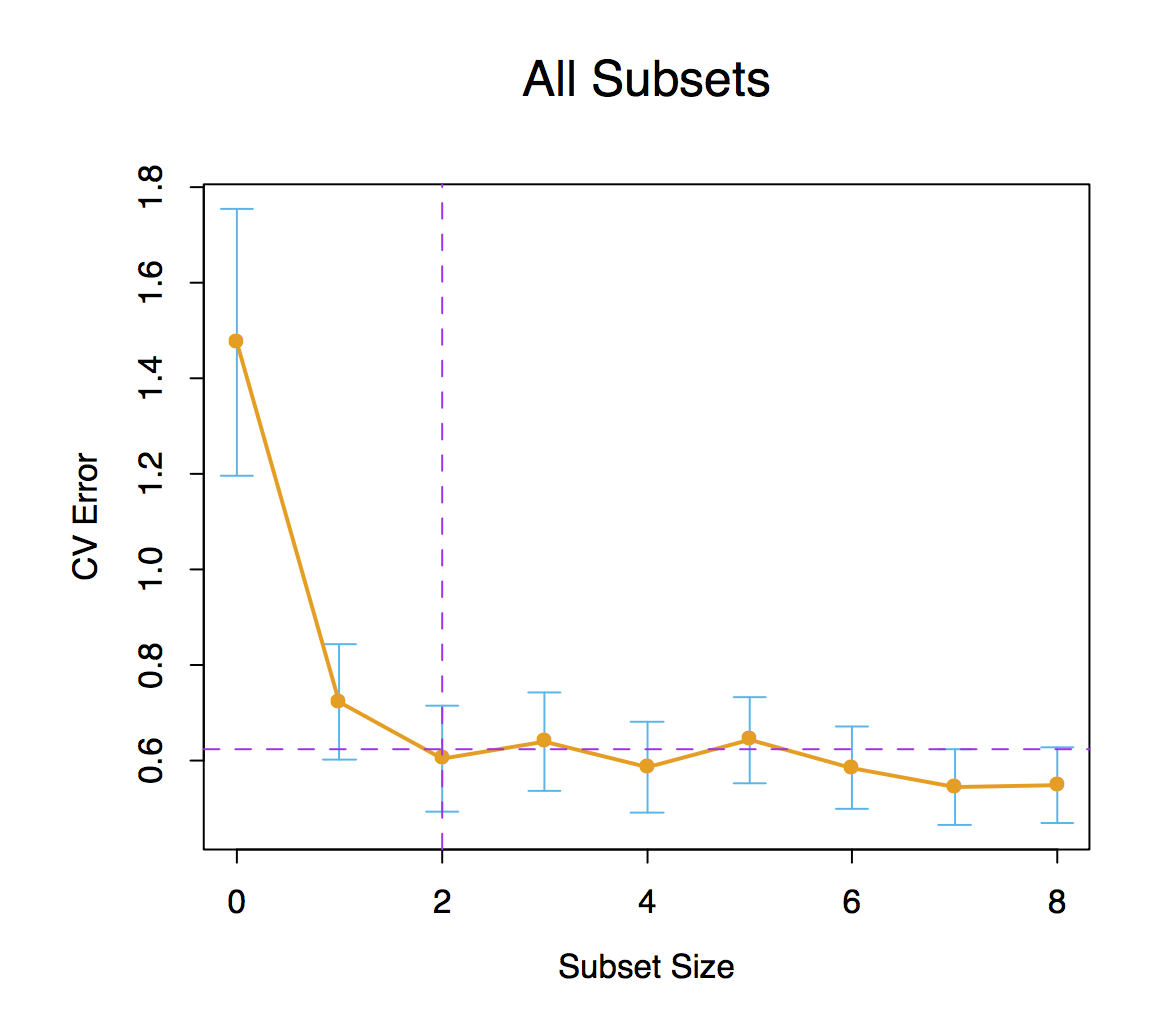
\includegraphics[width=0.6\textwidth]{all_subsets.png}
\caption{Prediction error curve using all subsets. Model complexity increases moving to the right.}
\end{figure}

\section{Shrinkage}
Subset Selection is very discrete. It's good for interpretation, but potentially (maybe not) bad for prediction.
\\
Shrinkage is a more continuous way to trade off more bias for less variance.
\\
\begin{center}
  $\hat{\beta}^{ridge}= argmin||Y-X_\beta||_2^2+\lambda\sum\limits_{j=1}^{p}\beta_{j}^2$
\end{center}
Shrinks $\hat{\beta}^{OLS}$ (the most complex linear model) foward sample mean of X (simplest prediction we can have)
\\
\\
At one extreme $\lambda$ = 0: $\hat{\beta}^{ridge} = \hat{\beta}^{OLS}$
\\
At other extreme $\lambda$ = $\infty$: $\hat{\beta}^{ridge}$ = intercept at sample mean of X
\\
\\
Shrinking to 0 prevents $\beta$ from trying to reach far off outliers with extreme slopes.
\\
\\
Rewrite $\lambda\sum\limits_{j=1}^{p}\beta_{j}^2$ = $\hat{\beta}^{T}\Lambda\beta$
where $\Lambda$ = $\bigl( \begin{matrix} 0 & \cdots & 0 \\ \lambda \\ & \ddots \\0 &&\lambda\end{matrix} \bigr)$ diagonal matrix	%BK: Is this right?
\\
So that... \\$\hat{\beta}^{ridge}= argmin(Y-X_{\beta})^T(Y-X_{\beta})+\beta^T\Lambda\beta$
\\
$\Delta((Y-X_{\beta})^T(Y-X_{\beta})+\beta^T\Lambda\beta) = -2X^T(Y-X_{\beta})+2\Lambda = 0$ %BK: Is it delta, or a gradient? \nabla?
\\$\Rightarrow X^TY = (X^TX+\Lambda)\beta$
\\$\Rightarrow \hat{\beta}^{ridge} = (X^TX+\Lambda)^{-1}X^TY$

\begin{figure}[H] 
\centering
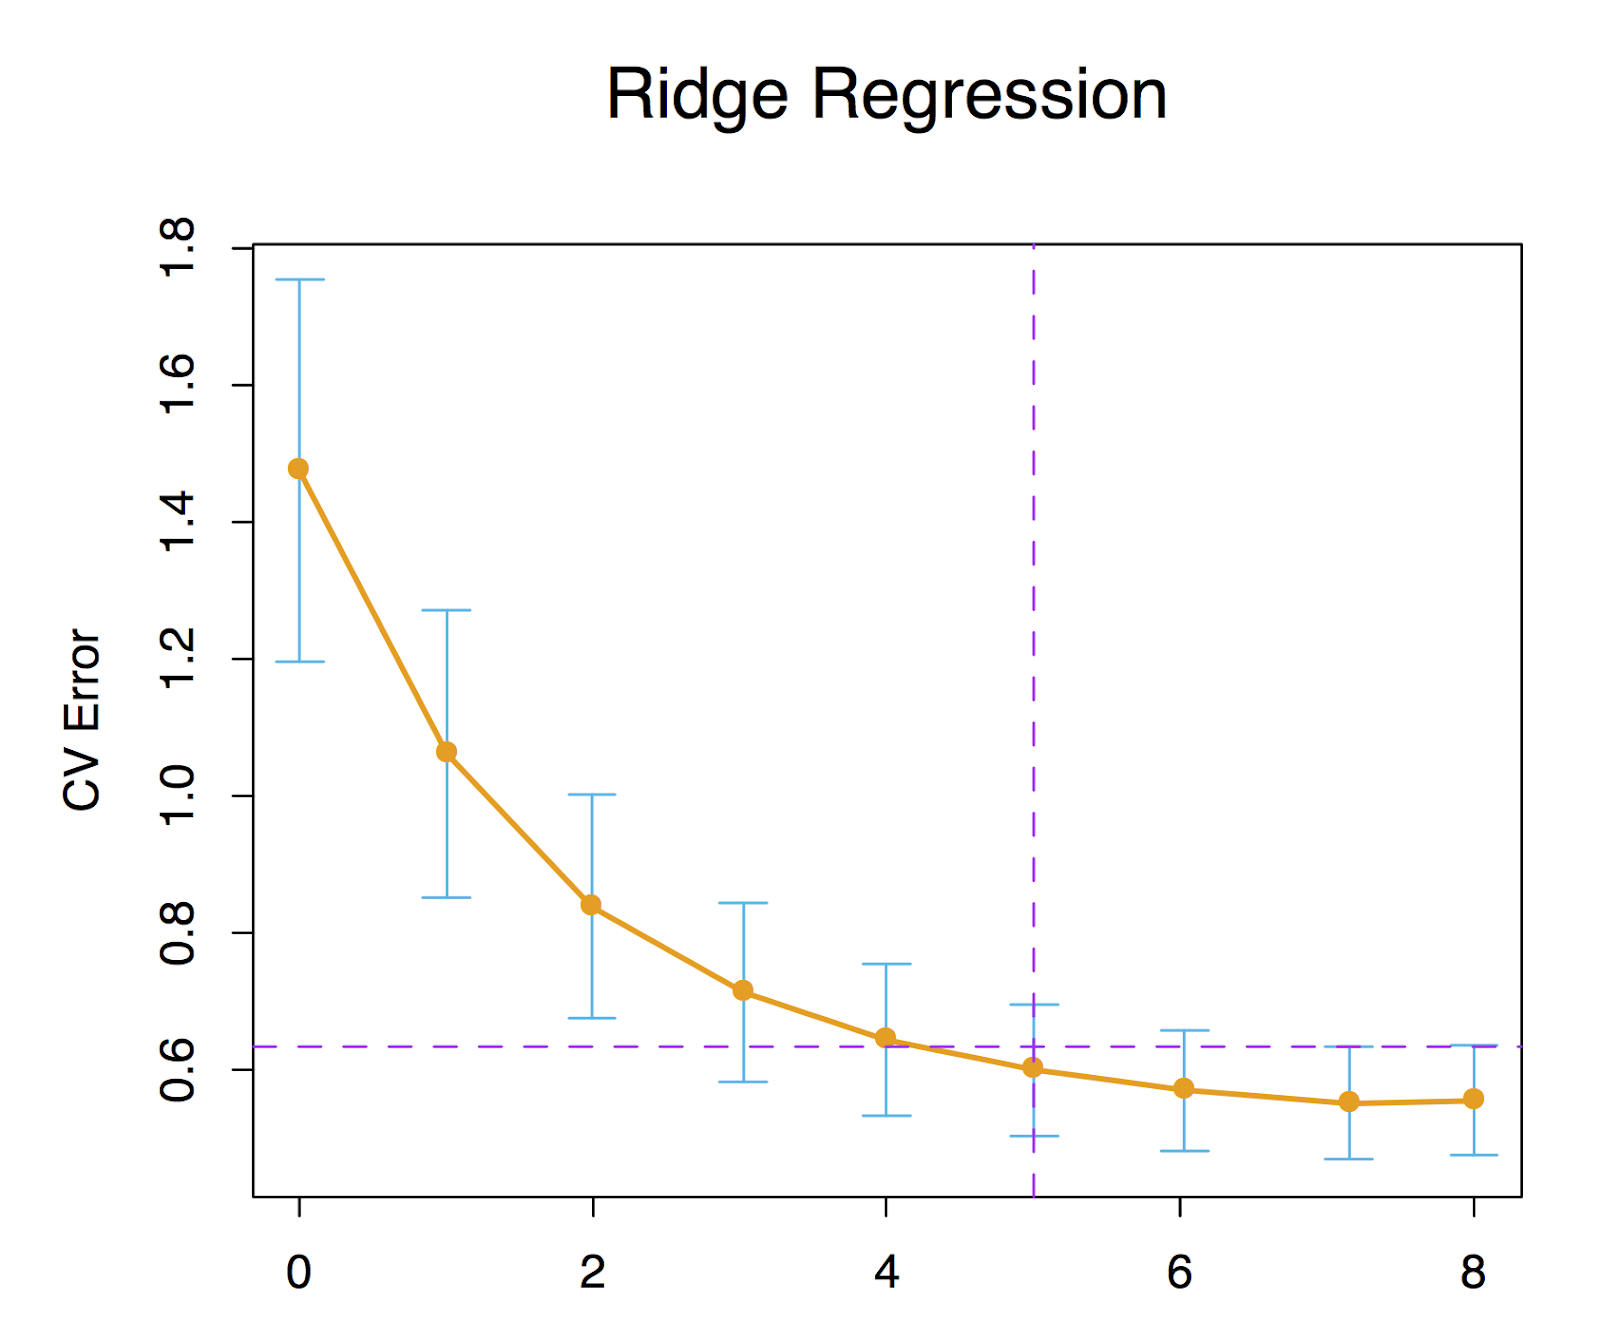
\includegraphics[width=0.6\textwidth]{ridge_regression.png}
\caption{Prediction error curve using ridge regression.}
\end{figure}

\begin{figure}[H] 
\centering
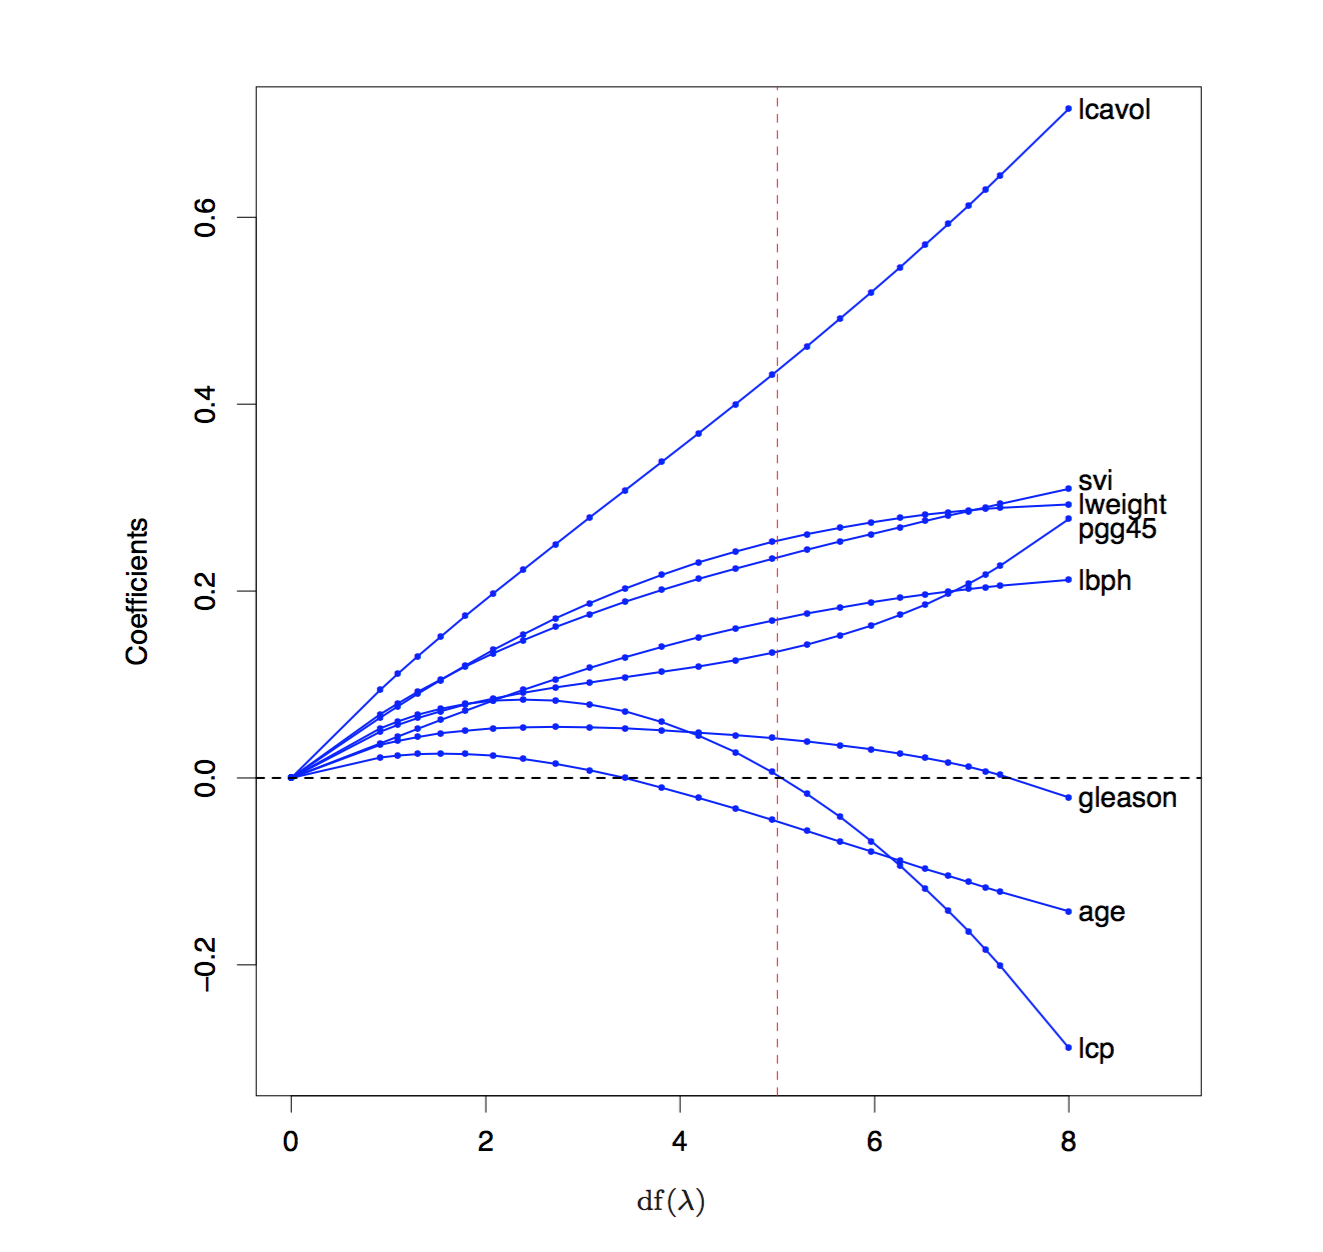
\includegraphics[width=0.6\textwidth]{ridge_regression2.png}
\caption{Ridge regression coefficients as determined by varying $\lambda$. Vertical line is chosen using cross validation}
\end{figure}

\section{Lasso Regression}
The idea behind Lasso Regression is to combine Shrinkage and Subset Selection
\\
\\
\begin{center}
  $\hat{\beta}^{Lasso} = argmin||Y-X_{\beta}||_2^2 + \lambda \sum\limits_{j=1}^{p} |\beta_{j}|$
\end{center}
Lasso, unike ridge and OLS, has no closed form solution. Fortunately, we can compute $\hat{\beta}^{Lasso}$ for all $\lambda$ simultaneously.
\\
\\
In sklearn, we can use:
\begin{center}
	sklearn.linear\textunderscore model.lasso\textunderscore path
\end{center}

\begin{figure}[H]
\centering
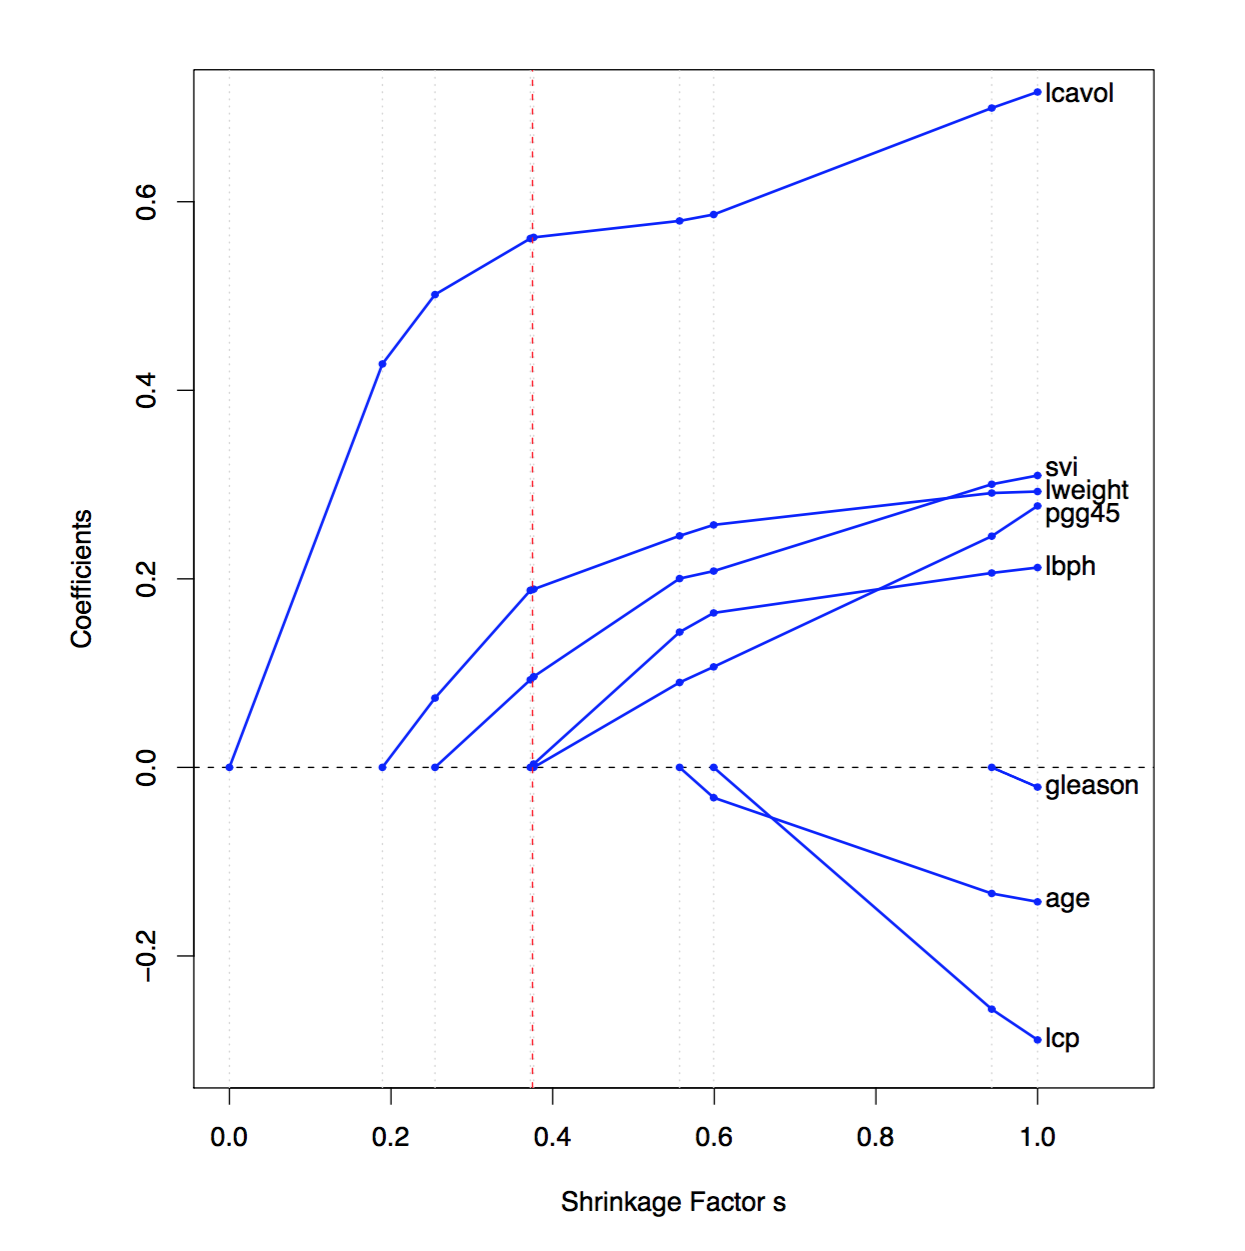
\includegraphics[width=0.6\textwidth]{lasso.png}
\caption{Lasso coefficients as determined by varying $\lambda$. Vertical line is chosen using cross validation}
\end{figure}

\begin{figure}[H]
\centering
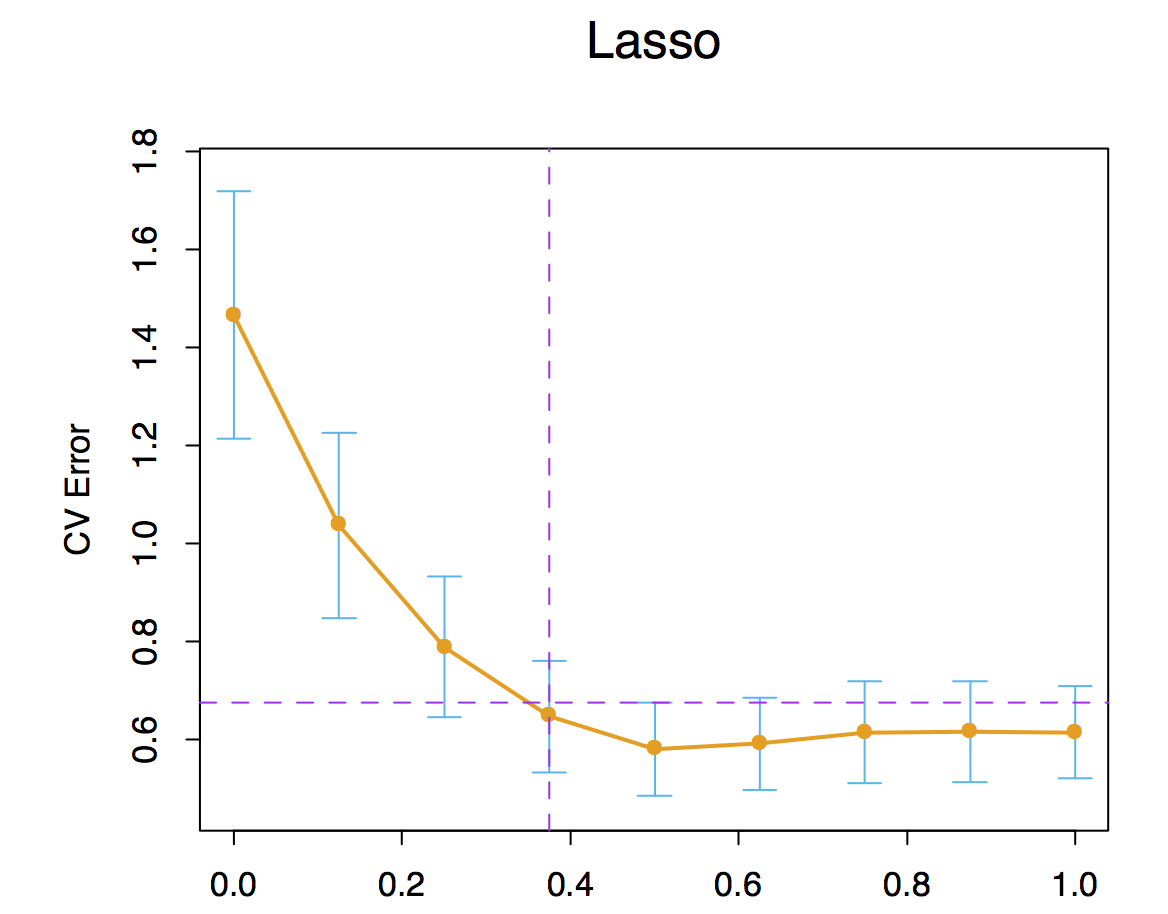
\includegraphics[width=0.6\textwidth]{lasso2.png}
\caption{Prediction error curve using lasso.}
\end{figure}

\end{document}